\chapter{Implementación}

\section{Control de versiones}
Para realizar un seguimiento del desarrollo de la aplicación se utilizará la
herramienta de control de versiones \textit{Git} \cite{git}, que permite llevar un
control de los cambios realizados en el código fuente de la aplicación. Además, estos
cambios se irán subiendo a la plataforma \textit{GitHub} \cite{github}.

Para seguir una estructura de los commits que se van realizando, se utilizará
el mensaje de commit con el formato "\texttt{<stack>} - \texttt{<mensaje>}", donde \texttt{<stack>}
es \textit{SERVER} o \textit{CLIENT} dependiendo de si el commit afecta al backend o
al frontend de la aplicación, y \texttt{<mensaje>} es la descripción de los cambios que
se han realizado.

En la figura \ref{fig:commits} se puede ver un ejemplo de una captura sacada
del listado de commits realizados en el repositorio de \textit{GitHub} \cite{github}.

\begin{figure}[H]
  \centering
  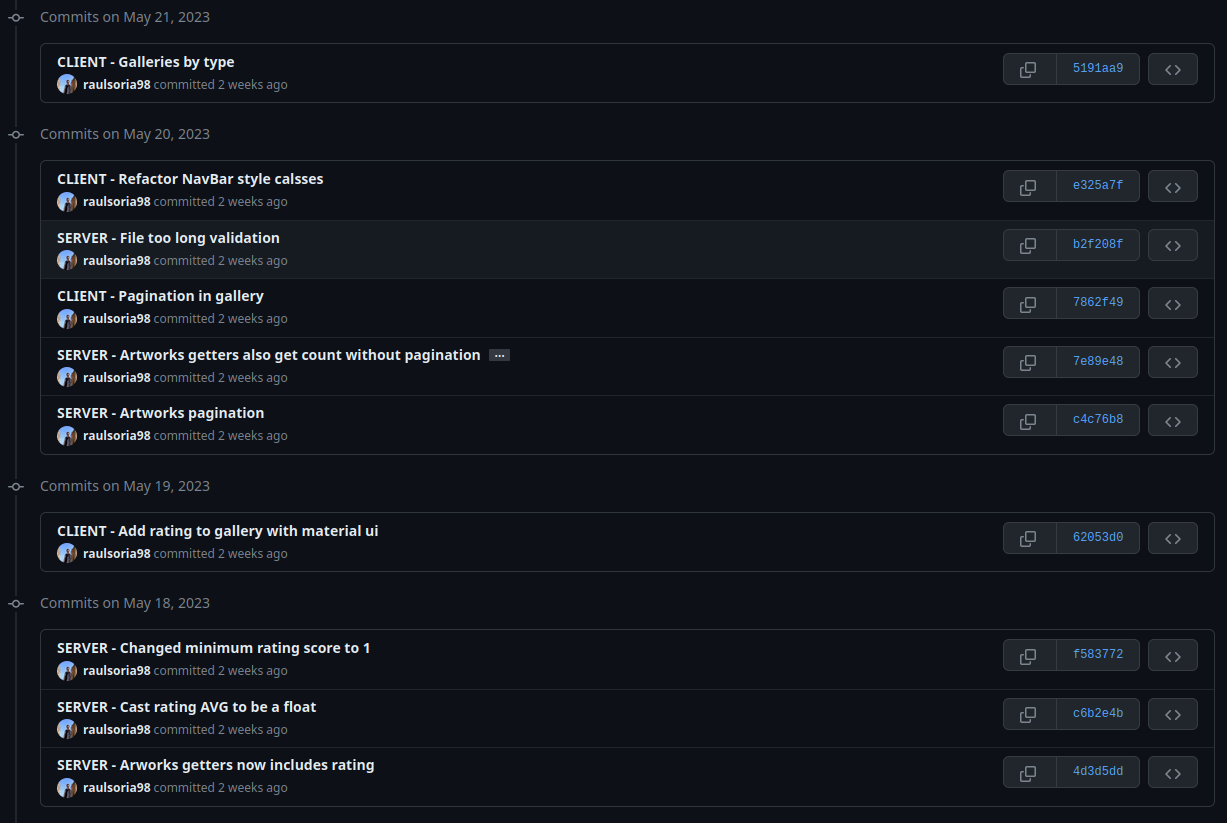
\includegraphics[width=1\textwidth]{commits}
  \caption{Ejemplo de mensajes de commit}
  \label{fig:commits}
\end{figure}
